\documentclass[10.5pt,a4paper]{article}
\usepackage[a4paper,margin=2cm]{geometry}
\usepackage[]{graphicx}
\usepackage{bm}
\usepackage{apacite}
\usepackage{url}
\usepackage{svg}
\usepackage{multirow}
\usepackage{amsmath}
\setlength{\parindent}{0pt}
\usepackage{pgf}
\usepackage{tikz}
\usepackage{pgfplots}
\usepackage{wrapfig}
\usepackage{float}
\usepackage[autostyle, english = american]{csquotes}
\usepackage[toc,page]{appendix}
\usepackage{amssymb}
\MakeOuterQuote{"}
\usepackage[T1]{fontenc}
\usepackage{enumitem}
\usepackage[none]{hyphenat}

\renewcommand{\baselinestretch}{1.1}
\setlist[enumerate]{itemsep=0mm}
\setlist[itemize]{itemsep=-0.7mm}
\begin{document}
	\nocite{*}
	
	\begin{titlepage}
		
		
		\title{Determining the effect of electrolyte concentration of the voltage produced by galvanic cells}
		
		\author{Noah Alexiou}
		
		
		\date{June 2025}
		
		\maketitle
		\centering
		
	\end{titlepage}
	\tableofcontents
	\newpage
	
	
	\section{Rationale}
	
	
	\subsection{Background}

	

	\textbf{Redox}
	
	Redox reactions are reactions that involve the transfer of electrons between atoms. These reactions commonly occur within galvanic cells, which within themselves contain two half cells. 
	

	\textbf{Half Cells}
	
	Half cells consists of an electrolyte solution and electrode. When two half cells are connected through a load, and a salt  bridge, one of these half cells will become the anode, where oxidation occurs, and the other will become the cathode, where reduction occurs. The oxidised cell will transfer its electrons across a wire, where they will then reach and be accepted by the reduced cell.
	
	Each half cell has its own standard electrode potential ($E^0$) which dictates the magnitude of electron emission, or attraction it has under standard lab conditions. This is also known as the `Voltage' of the cell
	
	By measuring the difference in magnitude between half cells, the overall potential between the cells can be quantified. \cite{GalvanicCellsCite}
	
	$$
	E^0_{\textrm{ Cell}}=E^0_{\textrm{ Cathode}}-E^0_{\textrm{ Anode}}
	$$
	
	For this experiment, the half cells will be made up of zinc and copper, which have $E^0$ values of $-0.7618$V, and $+0.3419$V respectively. Cell's with this composition are also known as "Daniell Cells", and will have a theoretical voltage, under standard conditions, of: 
	$$(0.3419-(-0.7618))=1.1037\textrm{V}$$
	
	\cite{StandardElectrodePotentialsCite}

	\textbf{The Nernst Equation}\newline
	The Nernst equation is a mathematical equation that allows the theoretical voltage potential of a cell to be quantified under non-standard conditions. While factors such as temperature and pressure throughout the experiment were not modified, the reaction quotient $(Q)$ was indirectly altered by the change in $[CuSO_4]$. 
\newline The Nernst equation is defined as:
	$$
	E_{\textrm{cell}}=E^0 - \frac{RT}{nF}\cdot \ln(Q)
	$$
	Where:
	\begin{itemize}
		\item $E$ = Theoretical electrode potential (voltage)of the cell
		\item $E^0$ = Standard electrode potential of the cell
		\item $T$ = Temperature in kelvin 
		\item $R$ = Universal gas constant
		\item $F$= Faraday constant
		\item $z$ = Number of moles of electrons transferred
		\item $Q$ = Reaction Quotient
		
\cite{NernstEquationCite}
	\end{itemize}
By substituting in constants for all values other than $[Cu^{2+}]$, the theoretical voltage can be found as a function of its concentration.  It should be noted that in this case, ${[CuSO_4]}$ and $[Cu^{2+}]$ are considered interchangeable terms, as the first is directly proportional to the latter.
\begin{align*}
E_{\textrm{cell}}=(0.3419+0.7618)-\frac{8.31446261815324\cdot298}{2\cdot96485}&\cdot\ln\frac{[Zn^{2+}]}{[Cu^{2+}]}\because \textrm{Constants and environmental conditions}\\
E_{\textrm{cell}}=(0.3419+0.7618)-\frac{8.31446261815324\cdot298}{2\cdot96485}&\cdot\ln\frac{1}{[Cu^{2+}]} \because [Zn^{2+}]\textrm{ remains constant}
\end{align*}

\begin{figure}

	\centering 

	

	\begin{tikzpicture}
		\begin{axis}[xmin=0, xmax=2, ymin=1.03, xlabel=${ \left[Cu^{2+}\right] }$, ylabel=$E_{\textrm{cell}}$, width=0.8\paperwidth, height=6cm]
			\addplot
		[
		samples=2000, smooth
		]
		{
				(0.3419+0.7618)-((8.31446261815324*298)/(2*96485))*ln(x^(-1))
		};
		\end{axis}
		
	\end{tikzpicture}
 
		\caption{The theoretical relationship between $E_{\textrm{cell}}$ and $[Cu^{2+}]$}
		\label{ogLog}
\end{figure}
\newpage
Considering Figure \ref{ogLog}, the theoretical change in $E_\textrm{cell}$ is minuscule in comparison to the change in $[Cu^{2+}]$. When the $x$-axis doubles from 0.5 to 1, a change of only $0.009$V is observed. If the relationship is further considered, with domain [0.5, 2], increasing concentration by a factor of 4 only results in an increase of $0.018$V. 
It was questioned whether this relationship held true, especially as $\lim\limits_{x\to 0}$.
As $Cu^{2+}$ increases from 0 to 1, it is theorised that the initial climb may appear more linear. If collision theory is considered, an increase in concentration is usually linearly proportional to the rate of reaction. When the concentration of ions is increased, more reactions should be able to take place per second, therefore increasing the output of the cell. It is hypothesised that at low concentrations, they may be too few ions in solution for the redox reaction to take place as expected. The concentration may rise linearly at low concentrations, but taper off as the reaction becomes `saturated'. The current model for this process was questioned.
\begin{figure}[h]
\begin{minipage}{0.5\textwidth}
	
	\begin{tikzpicture}
		\begin{axis}[ylabel=$E_\textrm{cell}$, xlabel=${[CuSO_4]}$]
			\addplot[] 		
			coordinates {
				(0, 0)
				(0.3, 1.15)
				(0.4, 1.15)
				(1, 1.15)
			};
			
		\end{axis}
	\end{tikzpicture}
	
\caption{Hypothesised relationship between $E_\textrm{cell}$ and $\left[CuSO_4\right]$	(Hypothetical graph to show expected shape. Axis numbers are to show increase in $x$ and $y$ axis, not predicted values.)}
\end{minipage}%
\begin{minipage}{0.001\textwidth}
	\hspace*{0.001cm}
\end{minipage}
\begin{minipage}{0.38\textwidth}
Investigation of $0<[Cu^{2+}]\leq1$ would theoretically be the most distinguishable from a logarithmic relationship if the observed trend diverges, due to the distinct curve observed in the area. 

Clearly $[Zn^{2+}]\neq 0$ and $[Cu^{2+}]\neq 0$, as this would either result in a division by 0, or $\ln(0)$, which both imply $E_\textrm{cell}=\textrm{undefined}$. Therefore $[CuSO_4]>0$ for the duration of the experiment so direct comparison could be made.
\vspace{2cm}
\end{minipage}
\end{figure}





\subsection{Research Question}
How does altering $[CuSO_4]$ at low concentrations (0.1-1 mol) affect its voltage output, and does the observed trend follow a linear relationship.
\section{Methodology}
\subsection{Modifications}

The following modifications were made to the original experiment. The original method can be found in the appendix section.\newline
\textbf{Half Cell Compositions}\newline
The results of original experiment indicated that copper and aluminium produced the largest voltage. It was theorised that after multiple trials, the aluminium would oxidise, skewing results.

It was decided that copper and zinc would be more suitable as although they produced a smaller voltage, zinc would take longer to oxidise and therefore producer more consistent results.

\textbf{Electrodes}\newline
Rather than thin strips, larger plates were bent into a "C" shape, slightly smaller than the diameter of the beaker they would be placed in. This maximised the surface area in contact with the electrolyte solution. Furthermore by reusing the same electrodes, this surface area was constant for all trials.

\textbf{Measurement devices}\newline
A digital multimeter was substituted in place of the conventional analog volt meter. Since the digital multimeter uses digital logic to measure voltage, rather than a magnetic field induced by the flow of current, the digital multimeter should reduce the ions 'used up' during each measurement. Furthermore the digital meter measures volts to 3 decimal places, leading to reduced uncertainty and increased precision. 

\textbf{Salt Bridge}\newline
The salt bridge was unaltered, and still made from filter paper, however, care was taken to ensure consistency in it's size.

\textbf{Procedure}\newline
The electrolyte solutions were pre-mixed, labelled, and stored in sealed containers prior to the start of the experiment. This reduced the potential for errors in procedure, as well as the time it took to conduct the experiment, which reduced the influence of environmental factors, such as changes in temperature, on results.
As previously mentioned, divergence from the Nernst equation would be more easily observable in the area of the vertical asymptote. Therefore the domain was limited to $0<[Cu^{2+}]\leq1$, and the density of measurements was increased as $\lim\limits_{[CuSO_4\rightarrow 0]}$.
\subsection{Method}
\textbf{Materials}
\begin{itemize}
	\item 30ml $CuSO_4$ at concentrations $1.00\textrm{M}, 0.85\textrm{M}, 0.70\textrm{M}, 0.55\textrm{M}, 0.40\textrm{M}, 0.30\textrm{M}, 0.20\textrm{M}, 0.10\textrm{M}$
	\item 240ml $1$M$\;ZnSO_4$
	\item 20ml $KNO_3$
	\item Petri dish
	\item $50\textrm{ml}$ Beaker - x$2$
	\item Zinc sheet $\approx4\textrm{cm}\times6\textrm{cm}$ 
	\item Copper sheet $\approx4\textrm{cm}\times6\textrm{cm}$ 
	\item Emery paper
	\item Filter paper strips $\approx 2\textrm{cm}\times10\textrm{cm}$
	\item Digital Multimeter
	\item Alligator clips
	\item 150ml Plastic bottle - x16
	\item Tweezers 
	\item 1L Distilled water
	\item Emery paper
\end{itemize}

\textbf{Procedure}
\small
\begin{enumerate}
	\item Pour varying amounts of $CUSO_4$ into 150ml plastic bottles and dilute with distilled water to form solutions with concentrations $1.00\textrm{M}, 0.85\textrm{M}, 0.70\textrm{M}, 0.55\textrm{M}, 0.40\textrm{M}, 0.30\textrm{M}, 0.20\textrm{M and } 0.10\textrm{M}$.
	
	\item Fill 8 of the 150ml plastic bottles with 30ml of 1M $ZnSO_4$ and set aside with copper solutions. 
	
	\item Polish electrodes with emery paper until they their entire surface is free of visible oxidation then connect to alligator clips.
	
	\item Connect alligator clips to multimeter and set to DC voltage mode.
	
	\item Transfer the contents of a $CUSO_4$, and $ZnSO_4$ container into separate beakers.
	
	\item Wet salt bridge with $KNO_3$ and rest over the lip of both beakers, so that it is partially submerged in both. 
	
	\item Add the electrodes to the solution and record result as soon as value settles.
	
	\item Remove electrodes immediately and wash with distilled water. Stir electrolyte solutions with a glass stir rod. Remove salt bridge and dispose of.
	
	\item Reconstruct cell with a new salt bridge, add electrodes back, and repeat measurementation so that there are three trials in total for any given concentration.
	
	\item Safely dispose of electrolyte solutions, wash equipment, and repeat for next $CuSO_4$ concentration.
\end{enumerate}

\subsection{Risk Assessment}
While the electrolytes utilised in this experiment are considered to be harmful if ingested or exposed to a persons eyes, there is no risk of injury via inhalation or accidental skin contact as long as appropriate action is taken (ventilation, washing affected area). PPE was worn by all participants to protect their eyes (lab goggles), body (lab coat) and hands (nitrite gloves). The electrolyte materials are  considered environmental hazar	content...ds ($CuSO_4, ZnSO_4$), however since the quantities used were so low, they could safely be disposed of in the sink after dilution.
\textit{For other risks or more details, see risk assessment table attached as an appendix.}

\section{Results}
\subsection{Results and Calculations}
\begin{figure}[h]
	\centering
\begin{tabular}{|c|c|c|c|c|c|}
	\hline
	[$CuSO_4$] & \multicolumn{3}{|c|}{Voltage}   & Mean & sigma \\
	\hline
	& Trial 1 & Trial 2 & Trial 3 &  &  \\
	\hline
	1 & 0.703 & 0.678 & 0.661 & 0.681 & 0.021 \\
	\hline
	0.85 & 0.664 & 0.623 & {\color{red} 0.488} & 0.592 & 0.088 \\
	\hline
	0.7 & 0.557 & 0.455 & 0.472 & 0.495 & 0.051 \\
	\hline
	0.55 & 0.457 & 0.422 & 0.413 & 0.431 & 0.022 \\
	\hline
	0.4 & 0.438 & 0.412 & 0.416 & 0.422 & 0.013 \\
	\hline
	0.3 & 0.498 & 0.47 & 0.476 & 0.481 & 0.014 \\
	\hline
	0.2 & 0.458 & 0.487 &  {\color{red}0.399} & 0.4725 & 0.0145 \\
	\hline
	0.1 & 0.405 & 0.456 & 0.463 & 0.441 & 0.029 \\
	\hline
\end{tabular}
\caption{Raw data with calculations. Outliers (highlighted in {\color{red} red}) \textbf{not} included in calculations}

\end{figure}
\begin{figure}[h]
	\centering
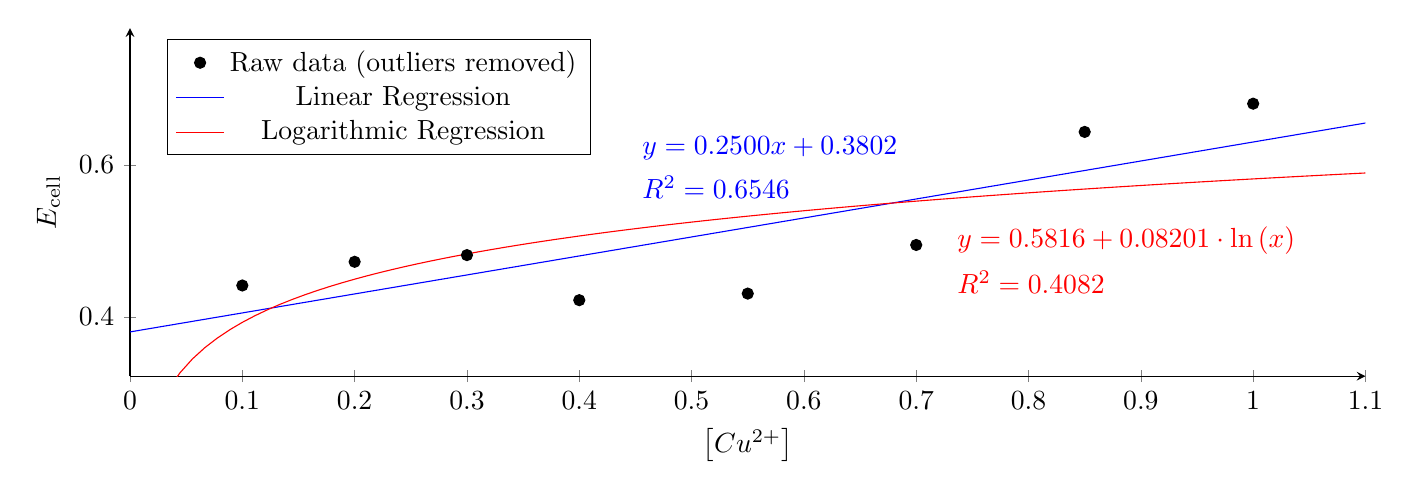
\begin{tikzpicture}
	\begin{axis}[xmin=0, xmax=1.1, ymin=0.322, ymax=0.78, axis lines=left, scale mode=stretch to fill, width=0.8\paperwidth, height=6cm, xtick distance=0.1, ytick distance=0.2, legend pos=north west, ylabel=$E_\textrm{cell}$, xlabel=${ \left[Cu^{2+}\right] }$]
		\addplot[only marks, mark=*, color=black]
		coordinates {
			(1, 0.680666666666667)
			(0.85, 0.6435)
			(0.7, 0.494666666666667)
			(0.55, 0.430666666666667)
			(0.4, 0.422)
			(0.3, 0.481333333333333)
			(0.2, 0.4725)
			(0.1, 0.441333333333333)
		};
		\addplot[no markers, blue, domain=0:1.1, samples=2, xlabel=] {0.250005837711617*x+0.38020534150613};
	\node [anchor=south west,inner ysep=3.8cm, inner xsep=6.5cm, color=blue] {$y=0.2500x+0.3802$};
	\node [anchor=south west,inner ysep=3.3cm, inner xsep=6.5cm, color=blue] {$R^{2}=0.6546$};
	
	
	\addplot[no markers, red, domain=0:1.1, samples=100, xlabel=] {0.0820068315129334*ln(x)+0.581619941927291};
	\node[anchor=south west,inner ysep=2.6cm, inner xsep=10.5cm, color=red]  {$y=0.5816+0.08201\cdot\ln\left(x\right)$};
	\node[anchor=south west,inner ysep=2.1cm, inner xsep=10.5cm, color=red]  {$R^{2}=0.4082$};
	
	
	
	
	\legend{Raw data (outliers removed), Linear Regression, Logarithmic Regression}

	\end{axis}
\end{tikzpicture}
\caption{Results (outliers removed) with linear, and logarithmic line of best fit.}
\label{RawLine}
\end{figure}

\newpage

\textbf{Finding Max and Min relationships}\newline
For $[CuSO_4]=1$mol\newline
\begin{align*}
	\sigma=&\pm\frac{\textrm{max}-\textrm{min}}{2}\\
	=&\pm\frac{0.703-0.661}{2}\\
	=&\pm0.021\\
	\\
	\textrm{Avg}=&0.6807\\
\end{align*}
For $[CuSO_4]=0.1$mol\newline
\begin{align*}
	\sigma=&\pm\frac{\textrm{max}-\textrm{min}}{2}\\
	=&\pm\frac{0.463-0.405}{2}\\
	=&0.029\\
	\\
	\textrm{Avg}=&0.4413\\
	&\\
	\textrm{Solve using linear regression between} &(\textrm{Avg}+\sigma, \textrm{Avg}-\sigma) \textrm{and}(\textrm{Avg}-\sigma, \textrm{Avg}+\sigma) \\
	\therefore \; \textrm{f(x)}_\textrm{Max}=0.3215 x& + 0.3802\\
	\textrm{f(x)}_\textrm{Min}=0.2104 x& + 0.4493
\end{align*}

\textbf{Finding Absolute Uncertainty in the Gradient}\newline
\begin{align*}
	\textrm{Considering }\sigma_\textrm{gradient}=&\pm\frac{\textrm{gradient}_\textrm{max}-\textrm{gradient}_\textrm{min}}{2}\\
	\sigma_\textrm{gradient}=&\pm\frac{0.3215-0.2104}{2}\\
	=&\pm0.05555\\
	\therefore\;\textrm{gradient}=\ \;&0.2500\pm0.05555
\end{align*}

\textbf{Finding Absolute Uncertainty in the $y$-intercept}\newline
\begin{align*}
	\textrm{Considering }\sigma_\textrm{$y$-int}=&\pm\frac{\textrm{$y$-int}_\textrm{max}-\textrm{$y$-int}_\textrm{min}}{2}\\
	\sigma_\textrm{$y$-int}=&\pm\frac{0.3802-0.4493}{2}\\
	=&\pm0.03455\\
	\therefore\;\textrm{$y$-int}=\;&0.3802\pm0.03455
\end{align*}

\textbf{Finding Percentage Uncertainty of the Gradient and $y$-intercept}\newline
\begin{align*}
	\textrm{\% uncertainty }=&\frac{\textrm{absolute uncertainty}}{\textrm{measurement}}\\
	\textrm{\% uncertainty}_\textrm{gradient}=&\frac{0.0556}{0.2500}\cdot100\\
	=&\;22.24\%\\
	\\
	\textrm{\% uncertainty}_\textrm{$y$-int}=&\frac{0.0346}{0.3802}\cdot100\\
	=&\;9.100\%\\
\end{align*}

\subsection{Analysis of Evidence}
\textbf{Identification of relationships and trends.}\newline
Across all trials, the voltage produced by the cell was lower than what the Nernst equation predicted. As $[CuSO_4]$ doubled from 0.1 to 0.2, the average $E_{cell}$ was scaled by a factor of 1.07. As it doubled again, from 0.2 to 0.4,  it was observed that the average $E_{cell}$  was scaled by a factor of $0.89$, which was smaller than the initial value. Clearly further investigation was required.
\vspace{.25cm}


The scatter plot produced using experimental data suggests a linear relationship. Using desmos, linear and logarithmic lines of best fit were found. Considering Figure \ref{RawLine}, the linear regression showed a greater correlation than the logarithmic.

$$R^2_\textrm{Lin}=0.6426>R^2_\textrm{Log}=0.4082$$


%Considering the components of the Nernst equation, it was considered that 
 %$$E_{\textrm{cell}}=(0.3419+0.7618)-\frac{8.31446261815324\cdot298}{2\cdot96485}\cdot\ln\frac{1}{[Cu^{2+}]}$$

The relationship between $[Cu^{2+}]$ and $E_\textrm{cell}$ was found to be linear, with a slope of $0.2500$, and vertical shift of $+0.3802$. The presence of vertical shift indicates divergence in the expected and actual relationships.  This is supported by theory, as when $\lim\limits_{[Cu^{2+}]\rightarrow 0}$, $E_\textrm{cell}\rightarrow 0$, as without another electrolyte facilitate the transfer of ions, the cell would have no potential. This suggests an incorrect hypothesis or error in procedure. Furthermore, it is unknown whether this relationship holds for higher $[Cu^{2+}]$ values. \cite{UCSBPhysicsCite} 


It should be noted that the data is limited, and does not perfectly match the linear model as the $R^2$ value is poor.
$$R^2_\textrm{Lin}=0.6546<1$$

\textbf{Analysis of Final Function}\newline
Considering the quantified uncertainties, the relationship between $[CuSO_4]$ and $E_\textrm{cell}$ was found to be:
$$E_\textrm{cell}=(0.2500\pm0.05555)x+(0.3802\pm0.03455)$$

The high percentage uncertainty in the gradient, $\approx22.24\%$, further suggests large errors in the experimental process. This implies that the relationship found is likely inaccurate. Overall while the data was inconsistent, it somewhat followed the theoretical linear relationship, however, the voltage `ceiling' was never reached, as data points kept increasing in value rather than plateauing.
\begin{figure}[h]
	
	\centering
	
	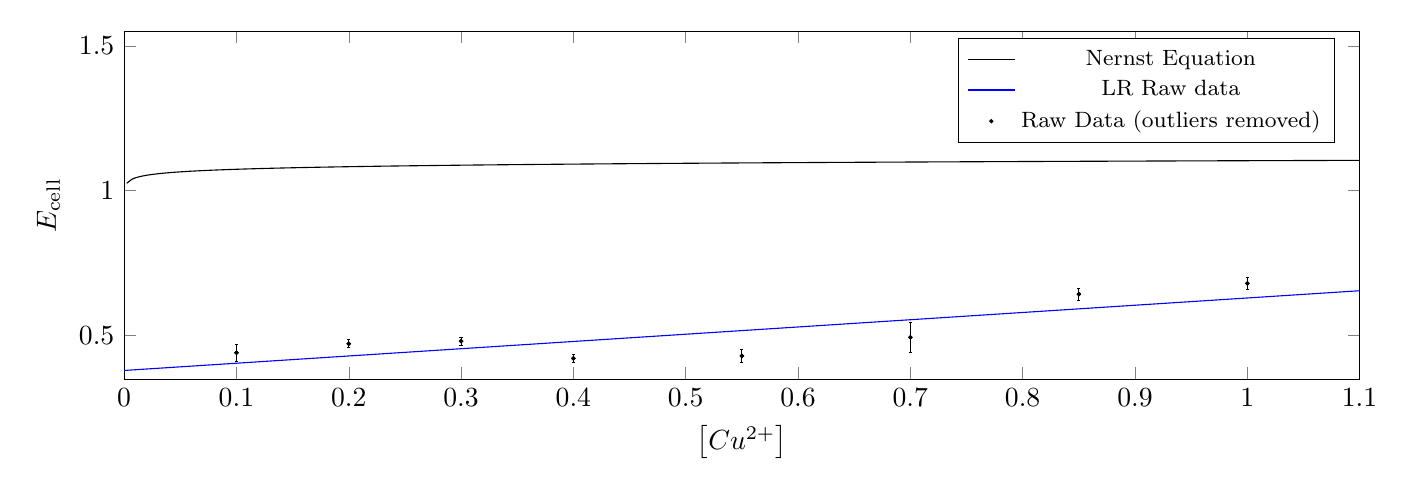
\begin{tikzpicture}
		\begin{axis}[xlabel=${ \left[Cu^{2+}\right] }$, ylabel=$E_{\textrm{cell}}$, width=0.8\paperwidth, height=6cm, xmin=0, ymin=0.35, xmax=1.1, ymax=1.55]
			\addplot
			[
			samples=2000, smooth
			]
			{
				(0.3419+0.7618)-((8.31446261815324*298)/(2*96485))*ln(x^(-1))
			};
			
			
					\addplot[no markers, blue, samples=2] {0.250005837711617*x+0.38020534150613};
					\addplot[only marks, mark=*, color=black, mark size=0.02cm]
		coordinates {
			(1, 0.680666666666667)
			(0.85, 0.6435)
			(0.7, 0.494666666666667)
			(0.55, 0.430666666666667)
			(0.4, 0.422)
			(0.3, 0.481333333333333)
			(0.2, 0.4725)
			(0.1, 0.441333333333333)
		};
			

		\legend{\footnotesize Nernst Equation, \footnotesize LR Raw data, \footnotesize Raw Data (outliers removed)}
		
		\addplot [
		 no markers, only marks , mark size=0.02cm,error bars,
		y dir=both,y explicit
		] coordinates {
			(1, 0.680666666666667) +- (0.021, 0.021)
			(0.85, 0.6435) +- (0.0205, 0.0205)
			(0.7, 0.494666666666667) +- (0.051, 0.051)
			(0.55, 0.430666666666667) +- (0.022, 0.022)
			(0.4, 0.422) +- (0.013, 0.013)
			(0.3, 0.481333333333333) +- (0.014, 0.014)
			(0.2, 0.4725) +- (0.0145, 0.0145)
			(0.1, 0.441333333333333) +- (0.029, 0.029)
				};
		
		\end{axis}
		
	\end{tikzpicture}
	
	\caption{The theoretical relationship between $E_{\textrm{cell}}$ and $[Cu^{2+}]$. (LR stands for Linear Regression)}
	\label{ogLog}
\end{figure}



\begin{figure}[h]

	\centering
\begin{tikzpicture}
	\centering
	\begin{axis}[xmax=3.1, xmin=0.9, ymax=0.8, ymin=0.3, width=0.82\paperwidth, scale mode=stretch to fill, height=8cm, axis lines=box, clip=false, legend style={font=\footnotesize}, legend style={at={(0.3, 0.94)}},  xtick distance=1, xlabel={Trial Number}, ylabel={Voltage}]
		
		\addplot [only marks, color=cyan,mark options={opacity=0.2}]
		coordinates{
		(1, 0.703)
		(1, 0.664)
		(1, 0.557)
		(1, 0.457)
		(1, 0.438)
		(1, 0.498)
		(1, 0.458)
		(1, 0.405)
	};

		\addplot [only marks, color=black, mark options={opacity=0.2}]
		coordinates{
		(2, 0.678)
		(2, 0.623)
		(2, 0.455)
		(2, 0.422)
		(2, 0.412)
		(2, 0.47)
		(2, 0.487)
		(2, 0.456)
	};

		\addplot [only marks, color=blue, mark options={opacity=0.2}]
		coordinates{
		(3, 0.661)
		(3, 0.488)
		(3, 0.472)
		(3, 0.413)
		(3, 0.416)
		(3, 0.476)
		(3, 0.463)		
		};
		

	    \addplot [
		error bars,
		y dir=both,y explicit
		] coordinates {
		(1, 0.5225) +- (0.149, 0.149)
		(2, 0.500375) +- (0.133, 0.133)
		(3, 0.484142857) +- (0.124, 0.124)		};



		\node[anchor=south west, inner ysep=4cm, inner xsep=8.7cm]{$y=-0.01925x+0.5408$};
		\node[anchor=south west, inner ysep=3.5cm, inner 	xsep=8.7cm]{$R^2=0.02712$};
			
	



		
		\legend{Trial 1 Results, Trial 2 Results, Trial 3 Results, LR of Average};
	\end{axis}
\end{tikzpicture}
\caption{Line of best fit for average voltage over sequential trials (outliers removed)}
\label{lowingVoltage}
\end{figure}
\newpage

\textbf{Considering the effects of electrolyte reuse}\newline
Figure \ref{lowingVoltage} depicts a trend observed where as trials continued, the voltage of each subsequent trial decreased slightly. Procedure was considered and it was theorised that this was due to reuse of the same electrolyte solution over multiple trials. The number of ions left on solution likely decreased as measurements were taken and and differed due to inconsistent duration of the measurement phase. This was theorised to have lead to a smaller voltage. To accurately consider this trend, and evaluate the reliability of the relationship, the average of all data points against what `trial' they were collected during was considered. While the change in voltage is only on average $-0.02$V per trial, considering $R^2=0.02712$, the linear regression indicates a very poor correlation. This was likely due to the large range of values considered for each `Trial Number'. therefore further investigation is required to confirm this. A far more reliable way to quantify this value would be measuring the decrease over number of trials while keeping the starting concentration constant.






\newpage
\section{Discussion}

\subsection{Sources of uncertainty and error}
\begin{center}
\centering
\begin{table}[]
	\resizebox{0.82\paperwidth}{!}{
\begin{tabular}{|l|l|l|}
	\hline
	\textbf{Observation}                                                                                                                         & \textbf{Source of error}                                                                                                                                                                                                                                                     & \textbf{Solution}                                                                                                                                                                                                                   \\ \hline
	\begin{tabular}[c]{@{}l@{}}Floating voltage on multimeter \\ in between trials. Voltage \\ fluctuation throughout trials.\end{tabular}       & \begin{tabular}[c]{@{}l@{}}Multimeter wires in contact with \\ puddle of electrolyte at \\ intermediate connection point \\ between meter and clips. \\ A minor redox reaction may \\ have been occurring on the bench, \\ affecting readings.\end{tabular}                  & \begin{tabular}[c]{@{}l@{}}Isolate multimeter from \\ experimental setup and ensure \\ probes are only connected to \\ electrodes.\end{tabular}                                                                                     \\ \hline
	\begin{tabular}[c]{@{}l@{}}Inconsistent voltage readings \\ and high electrolyte consumption \\ over relatively short readings.\end{tabular} & \begin{tabular}[c]{@{}l@{}}Alligator clips of unknown material \\ were submerged in the half cells\\ electrolyte solution. Likely \\ dissociating and affecting half cell \\ composition unintentionally.\end{tabular}                                                       & \begin{tabular}[c]{@{}l@{}}Alter shape of electrodes to a \\ portion of it extends beyond \\ the edge of the beaker so that \\ alligator clips can be attached \\ without being at risk of \\ contacting electrolytes.\end{tabular} \\ \hline
	Large voltage drops between trials.                                                                                                          & \begin{tabular}[c]{@{}l@{}}Inconsistent measurement times and \\ gaps between trials. During some trials,\\ the multimeter disconnected midway \\ through measurement and when reconnected \\ the voltage reading was significantly lower \\ than other trials.\end{tabular} & \begin{tabular}[c]{@{}l@{}}Perform all step-lens at set time \\ intervals. Take care to ensure \\ setup remains the same \\ throughout all trials.\end{tabular}                                                                     \\ \hline
	Consistently lower voltages than expected.                                                                                                   & \begin{tabular}[c]{@{}l@{}}Unknown. Possibly resistance due to \\ small salt bridge or poor wiring, oxide \\ layer on electrodes, incorrect electrolyte \\ concentrations.\end{tabular}                                                                                      & \begin{tabular}[c]{@{}l@{}}Follow procedure with more \\ care. Use more suitable \\ equipment.\end{tabular}                                                                                                                         \\ \hline
	\begin{tabular}[c]{@{}l@{}}Estimated Nernst equation\\ values\end{tabular}                                                                   & \begin{tabular}[c]{@{}l@{}}Environmental conditions were\\ not measured during the experiment.\\ This would result in very slight changes\\ in the Nernst equation's value for\\ any given trial.\end{tabular}                                                               & \begin{tabular}[c]{@{}l@{}}Record environmental \\ conditions. (Temperature,\\ Pressure)\end{tabular}                                                                                                                               \\ \hline
	Unknown impact of reusing electrolyte.                                                                                                       & \begin{tabular}[c]{@{}l@{}}Not enough trials performed\\ using same electrolyte for\\ reliable relationship to be \\ quantified.\end{tabular}                                                                                                                                & \begin{tabular}[c]{@{}l@{}}Repeat for many trials to\\ measure decrease in voltage \\ to quantify and account for \\ change or use fresh \\ electrolyte for each trial.\end{tabular}                                                 \\ \hline
\end{tabular}
}
\end{table}

\end{center}




\subsection{Extensions}

	Galvanic cells have properties other than voltage ($V$), such as resistance ($R$), current output ($I$), and overall power ($W$). It is possible that altering the concentration of the cell has an greater impact on these attributes, as opposed to voltage alone. This is supported by Ohms law, which states that $V=I\cdot R$. A possible extension to this experiment could investigate the effects of varying electrolyte concentration on these characteristics of a galvanic cell.
	\newline
	
	It was noticed that the Nernst equation does not take into account the actual concentrations of electrolyte solutions, but merely the ratio between them, in the form of the reaction quotient ($Q$)
	\begin{align*}
\because E_{\textrm{cell}}=&E^0 - \frac{RT}{nF}\cdot \ln(\mathbf{Q})\\
\mathbf{Q}=&\frac{[Zn^{2+}]}{[Cu^{2+}]}
	\end{align*}

Theoretically, a cell with equally highly concentrated electrolyte solutions will experience ion flow differently to a cell with very low concentrations. Another possible extension to this experiment could be the investigation of cell properties as the concentration of both electrolyte solutions approach $0$.
	




\section{Conclusion}
This experiment investigated the effect of altering $[CuSO_4]$ at low concentrations (0.1-1 mol) affect its voltage output, and whether observed trend followed a linear relationship.  Overall the research question was answered, and it was found that while the results most closely followed the hypothesised linear relationship, they were unreliable and poorly correlated. The cell voltages were lower than expected throughout all trials, which suggested the presence of inefficiencies or errors in the experimental setup and processes such as contamination and multiple instances of mistakes causing there to be major outliers in the dataset. Solutions to improve the experiments design, such as better isolation and procedure design, and extensions, such as further investigation into cell power output and other properties under varying conditions, were suggested.
\section*{Appendices}

\subsection*{Risk Assessment}
\begin{figure}[h]
	
	\tiny
	\begin{tabular}{|p{3cm}|p{4cm}|p{4.5cm}|p{4cm}|}
		
		\hline
		\textbf{Item/Substance} & \textbf{Potential Hazards} & \textbf{Standard Handling Procedures} & \textbf{Disposal} \\
		\hline
		Alligator clip with lead & Clip may cause pain and injury if applied to skin. & & \\
		\hline
		Glass beaker & Breakage of beaker. Cuts from chipped rims. & Inspect and discard any chipped or cracked beakers. Sweep up broken glass with brush and dustpan; do not use fingers. & \\
		\hline
		Metal tweezers & Can be used as a weapon if long and sharply pointed. & & \\
		\hline
		Disposable plastic gloves & May easily be punctured, allowing entry of liquid. Latex gloves may cause an allergic reaction to some people& Take care not to puncture. Check for punctures before use. Use a type of glove that is suitable for the chemicals to be used. & \\
		\hline
		Lab coat & \textbf{Flammable}. Sleeves may catch on objects and knock them over. & & \\
		\hline
		Safety glasses & Scratched or dirty glasses may hinder vision, causing headaches during prolonged use. & \textbf{Each person should preferably have own safety glasses}. Check and, if necessary, clean glasses before each use.. & \\
		\hline
		Filter paper & \textbf{Flammable}. \textbf{Used filter paper may contain harmful residues}. & After use, dispose of residue and filter paper appropriately. & Dispose of residue and filter paper appropriately. \\
		\hline
		Copper (sheet) & Not toxic. & & $<$1 kg/day may be placed in the garbage. Larger quantities should be retained for collection by a waste service or metal recycler. \\
		\hline
		Copper(II) sulfate ($>$0.94 M) & \textbf{Toxic}. \textbf{Irritates skin and eyes}. & $<$5 mL/day may be poured down the drain. Larger quantities should be placed in a Copper waste container. &\\
		\hline
		Zinc (pieces) & Not toxic to humans. & & \textbf{May be placed in the garbage}. \\
		\hline
		Zinc nitrate (0.79-1 M) & \textbf{Toxic}. \textbf{Irritates skin, eyes and lungs}. \textbf{Harmful if swallowed}. Causes skin irritation. \textbf{Causes serious eye irritation}. \textbf{Very toxic to aquatic life with long lasting effects}. & & $<$5 mL/day may be diluted with 10 times the volume of water and poured down the drain. Larger quantities should be placed in a Zinc waste container. \\
		\hline
		Potassium nitrate (0.1-1 M) & \textbf{May irritate eyes and skin}. GHS data: Not classified as a hazardous chemical. & & $<$1 L/day may be poured down the drain in a stream of water. \\
		\hline
		Wash bottle & May be used to spray others. & Preferably use distilled water. Change water regularly to avoid microbial growth. & \\
		\hline
	\end{tabular}
	\normalsize
\end{figure}





\bibliography{refrences.bib}
\bibliographystyle{apacite}
\nocite{*}

\end{document}
